\documentclass[11pt,a4paper]{article}
\usepackage{xcolor}
%\usepackage[german]{babel}
\usepackage[T1]{fontenc}
\usepackage{amsmath}
\usepackage{amsfonts}
\usepackage{amssymb}
\usepackage{graphicx}
\usepackage{enumitem}
\usepackage{subcaption}%\begin{subfigure}{Breite der Subfigure}
\usepackage[left=3cm,right=3cm,top=2cm,bottom=2cm]{geometry}
\usepackage{physics}
\title{Coursework 2 - Modern Computational Techniques \vspace{-1.5cm}}
\date{}
%\author{Sebastian Kock}
\begin{document}
\maketitle
\newcommand{\num}{\thenum \stepcounter{num} }
\newcommand{\aufgabe}[1]{\subsection*{Aufgabe A\thesubsection: #1}
    \stepcounter{subsection}}
% \setcounter{section}{•}
\setcounter{subsection}{1}
\newcommand{\enumalph}{\renewcommand{\theenumi}{\alph{enumi}}}

\section*{Description Q1 }
\subsection*{Neural Network Structure}
For the memorisation of the 3-input XOR gate, a perceptron with a single hidden
layer is trained in \texttt{NN\_metropolis.py}. Since no generalisation of the
training data is intended, the hidden layer could have as many nodes as
computationally sensible. As overfitting is favourable in our case,
the hidden layer of the used neural network (NN) has 5 nodes, set by the
variable
\texttt{nhidden}. According to the given data, NN has 3 input nodes and
one node in the output layer. A bias node that has always value 1 is attached
to input and hidden layer, to improve generalisation performance. Therefore
the bias node is not connected to the input layer. The resulting layout can
is shown in figure \ref{fig:struct}.

\begin{figure}[h]
    \centering
    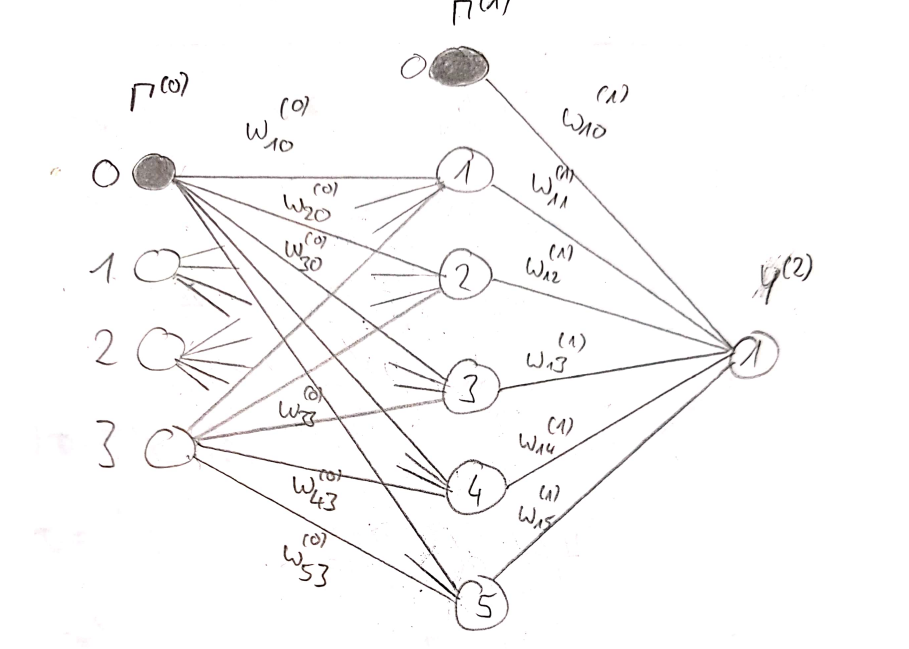
\includegraphics[width=0.7\textwidth]{NN.png}
    \caption{Chosen Neural Network Structure}
    \label{fig:struct}
\end{figure}

In the submitted program the shape of the NN is determined by the shape of
the provided weight arrays. Each weight $w_{ij}^{(n)}$ can be described by the 
three indices
\begin{align*}
    n \in \{0,1\} \ &: \quad \text{layer index} \\
    i \ &: \quad \text{output node index} \\
    j \ &: \quad \text{input node index}
\end{align*}
As a result the corresponding weight matrices for each layer $(\mathbf{W}^{(n)})_{ij}$ 
are of the vector spaces
\begin{align}
    \mathbf{W}^{(0)}\in \mathbb{R}^{5\cross 4} \quad \text{and} \quad 
    \mathbf{W}^{(1)}\in \mathbb{R}^{1\cross 6}
\end{align}
which also includes the bias weight into the matrix. This definition requires that
the 3 dimensional input vector $Y^{(0)}$ from the truth table is extended by the bias
to
\begin{equation*}
    \Gamma^{0} = \left( 1,  Y^{(0) T} \right)^T
\end{equation*}
so that the output of the first layer can be written as
\begin{equation}
    Y^{(1)} = \sigma(\mathbf{W^{(0)}} \Gamma^{(0)} ) .
\end{equation}
The activation function $\sigma(x) = \frac{1}{1+\exp(-x)}$ is defined element wise on 
vectors. Generalising this gives
\begin{equation}
    Y^{(n)} = \sigma(\mathbf{W^{(n)}} \Gamma^{(n)} ) .
\end{equation}
In the code, the training samples are all contained in a single matrix with
each row corresponding to the inputs of the truth table. That means that 
each input vector $Y_k$ of row k is implemented as row of the new matrix. With numpy
this makes the code more efficient.

\subsection*{Metropolis Algorithm Implementation}
The implemented Metropolis Algorithm minimises the sum of squared error of all inputs.
The inverse temperature $\beta$ is set to an initial value \texttt{beta} and is 
increased linearly in steps of \texttt{betastep} after \texttt{eqiter} iterations.
After \texttt{maxiter} updates of $\beta$, the algorithm is stopped without result.

The algorithm starts with random weights in the range $\left[-1, 1\right]$.
In each iteration one weight is selected randomly and changed by a random amount
$\Delta w \in \left[-\alpha, \alpha\right]$. Each random choice is drawn from a uniform 
distribution. The metropolis algorithm decides then in the given randomised form
if the changed weight is accepted or not.

The used values for the parameters in the code proved most effective in obtaining
a trained NN as fast and reliable as possible. However, there are cases in which the
algorithm does not find a minimum that corresponds to a trained NN.

\end{document}